\section{Embasamento Teórico}
    \label{sec:emb_teo}
A computação evolutiva adapta a teoria evolutiva do Darwinismo à automatização da solução de problemas. Consiste, basicamente, em considerar uma população de indivíduos que crescerão, tendo sua adaptação ao ambiente avaliada, e passarão pela pressão da seleção natural. Os indivíduos mais ajustados poderão ser utilizados como semente na próxima geração~\cite{EIBEN20021}.

Há diversos conjuntos de regras dentro da computação evolutiva como: algoritmos genéticos, estratégias evolutivas, programação evolutiva e programação genética. Algoritmos genéticos é o conjunto utilizado neste projeto.

\subsection{Algoritmo Genético}
    \label{subsec:emb_teo_alg_gntc}
Conjunto da computação evolutiva que utiliza a representação de sequência de~\emph{bits}, aplicando troca ou mudança de ~\emph{bits} como suas operações~\cite{EIBEN20021}.

Os indivíduos, que podem ser chamados de~\emph{cromossomos}, é composto por~\emph{genes} que armazenam grande significado em seu valor e na sua posição, onde uma alteração pode mudar completamente esse indivíduo. Além dos~\emph{bits}, inicialmente propostos, como genes outras estruturas podem ser utilizadas, adaptando-se ao problema que deseja ser resolvido.

\begin{figure}[!ht]
    \centering
    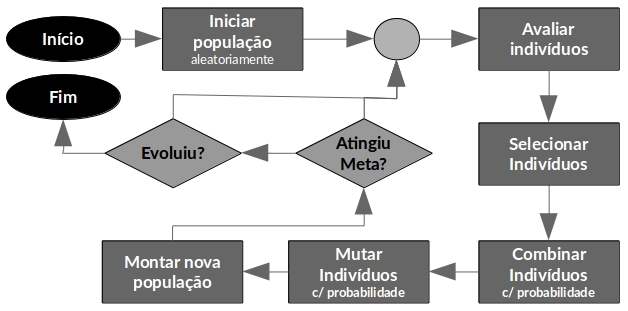
\includegraphics[width=\linewidth]{Imagens/Genetic_algorithm_steps.png}
    \caption{Etapas presente no algoritmo genético.}
    \label{fig:emb_alg_gntc_etapas}
\end{figure}

Conforme ilustrado na Figura~\ref{fig:emb_alg_gntc_etapas}, um algoritmo genético têm as seguintes etapas:

\begin{enumerate}
    \item \textbf{Inicialização da população:} uma quantidade $\mathcal{N}$ de indivíduos é gerada aleatoriamente, respeitando a configuração dos cromossomos;
    \item \textbf{Avaliação dos indivíduos:} assim como na teoria do evolucionismo, os indivíduos possuem sua adaptabilidade ao ambiente avaliada e mensurada e, então, utilizada para ordenação da população. Esta avaliação dos indivíduos está intrinsecamente vinculada ao problema em questão e deve ser avaliada como tal;
    \item \textbf{Seleção de indivíduos:} com os dados referentes à adaptação dos indivíduos, somente os mais aptos podem ser selecionados para proliferar;
    \item \textbf{Combinação de indivíduos:} com os mais adaptados separados ou não, os genes de um par de indivíduos são combinados de forma a trocar dados e poder gerar novos indivíduos;
    \item \textbf{Mutação de indivíduos:} ainda considerando os mais adaptados ou não, os indivíduos possuem seus genes alterados internamente e pode gerar novos indivíduos;
    \item \textbf{Montagem de uma nova população:} considerando a população atual, ou os indivíduos mais adaptados, e os indivíduos gerados, uma nova população é configurada e estará disponível como a próxima geração;
    \item \textbf{Avaliação dos critérios:} este algoritmo poderia ser executado infinitivamente, mas como uma resposta está sendo esperada, critérios de parada devem ser definidos. Caso sejam alcançados: a última geração é considerada como provável portadora da resposta desejada; caso contrário, o processo é repetido a partir da~\textbf{Avaliação dos indivíduos}.
\end{enumerate}

Vale ressaltar que a~\textbf{Avaliação dos critérios} informou que ``a última geração é considerada como~\emph{provável} portadora da resposta desejada'', por se tratar de uma busca pelo caso médio, não pelo melhor caso.

Embora todas as etapas tenham detalhes e minúcias, apenas a combinação e a mutação serão detalhadas. Para tanto, serão considerados cromossomos com $10$ genes inteiros de $0$ a $9$, tendo o $9$ como fixo na posição $\mathbf{0}$, conforme demonstrado na Tabela~\ref{tab:emb_alg_gntc_exemplo_xsomo}.

% Criada usando: https://www.tablesgenerator.com/latex_tables#
\begin{table}[!h]
    \centering
    \begin{tabular}{>{\columncolor[HTML]{656565}}l |c|c|c|c|c|c|c|c|c|c}
        \cline{2-11}
        \rowcolor[HTML]{C0C0C0}
        \cellcolor[HTML]{FFFFFF} & $\mathbf{0}$ & $\mathbf{1}$ & $\mathbf{2}$ & $\mathbf{3}$ & $\mathbf{4}$ & $\mathbf{5}$ & $\mathbf{6}$ & $\mathbf{7}$ & $\mathbf{8}$ & $\mathbf{9}$ \\ \hline
        {\color[HTML]{FFFFFF} $I_1$} & 9 & 4 & 6 & 0 & 1 & 2 & 7 & 5 & 8 & 3 \\ \hline
    \end{tabular}
    \caption{Exemplo de cromossomo de $10$ genes inteiros de $0$ a $9$.}
    \label{tab:emb_alg_gntc_exemplo_xsomo}
\end{table}

\subsection{Combinação}
    \label{subsec:emb_teo_xover}
Quanto maior o cromossomo maiores as possibilidades de métodos para realizar a combinação de genes de dois indivíduos, eis algumas possibilidades:

\begin{itemize}
    \item \textbf{Combinação de 2 pontos:} dados dois indivíduos ($I_1$ e $I_2$), duas posições de seus genes são sorteadas. Os genes fora do intervalo entre as posições serão copiados de $I_1$ para o filho $F_1$ e de $I_2$ para o filho $F_2$. Já os genes dentro do intervalo serão copiados de $I_2$ para $F_1$ e de $I_1$ para $F_2$, sendo verificado se o gene a ser copiado não está presente na parte fixa do filho, e, caso esteja, o filho mantém o gene do pai que forneceu sua parte fixa - adaptado~\cite{stoltz_2018}. Após as trocas de genes, ainda é possível haver duplicatas na região contida entre as posições sorteadas, isso é tratado substituindo um dos genes repetidos pelo gene não presente no filho - adaptado~\cite{ferreira_2007}. Exemplificando na Tabela~\ref{tab:emb_teo_xover_2point}, as posições sorteadas foram a $\mathbf{4}$ e a $\mathbf{7}$, então os genes das posições de 0 a 3 e de 8 a 9 (em negrito) serão fixos nos filhos $F_1$ e $F_2$, que recebem os genes fixos de $I_1$ e $I_2$ respectivamente. Os genes entre as posições 4 e 7 foram trocados evitando-se repetição com os genes fora desse intervalo (no exemplo, não houve troca nas posições que contém gene sublinhado, que, caso fosse trocado, geraria duplicação com gene fixo). No exemplo, ocorreu repetição entre genes dentro do intervalo e, com isso, um dos genes repetidos foi substituído pelo gene não presente no filho, como podemos observar na posição 5 de $F_1$, onde ocorreu repetição do gene 1 que foi substituído por 3, e na posição 4 de $F_2$, onde ocorreu repetição do gene 3 que foi substituído por 1.
        \begin{table}[!h]
            \centering
            \begin{tabular}{>{\columncolor[HTML]{656565}}l |c|c|c|c|c|c|c|c|c|c}
                \cline{2-11}
                \rowcolor[HTML]{C0C0C0}
                \cellcolor[HTML]{FFFFFF} & $\mathbf{0}$ & $\mathbf{1}$ & $\mathbf{2}$ & $\mathbf{3}$ & $\mathbf{4}$ & $\mathbf{5}$ & $\mathbf{6}$ & $\mathbf{7}$ & $\mathbf{8}$ & $\mathbf{9}$ \\ \hline
                {\color[HTML]{FFFFFF} $I_1$} & 9 & \cellcolor[HTML]{B34040}{\color[HTML]{FFFFFF} 2} & \cellcolor[HTML]{B34040}{\color[HTML]{FFFFFF} 0} & \cellcolor[HTML]{B34040}{\color[HTML]{FFFFFF} 4} & 3 & 7 & 5 & 1 & \cellcolor[HTML]{B34040}{\color[HTML]{FFFFFF} 8} & \cellcolor[HTML]{B34040}{\color[HTML]{FFFFFF} 6} \\ \hline
                {\color[HTML]{FFFFFF} $I_2$} & 9 & \cellcolor[HTML]{44B340}{\color[HTML]{FFFFFF} 5} & \cellcolor[HTML]{44B340}{\color[HTML]{FFFFFF} 2} & \cellcolor[HTML]{44B340}{\color[HTML]{FFFFFF} 4} & 7 & 1 & 3 & 6 & \cellcolor[HTML]{44B340}{\color[HTML]{FFFFFF} 0} & \cellcolor[HTML]{44B340}{\color[HTML]{FFFFFF} 8} \\ \hline
                {\color[HTML]{FFFFFF} $F_1$} & 9 & \cellcolor[HTML]{B34040}{\color[HTML]{FFFFFF} 2} & \cellcolor[HTML]{B34040}{\color[HTML]{FFFFFF} 0} & \cellcolor[HTML]{B34040}{\color[HTML]{FFFFFF} 4} & 7 & \sout{1} 3 & \underline{5} & 1 & \cellcolor[HTML]{B34040}{\color[HTML]{FFFFFF} 8} & \cellcolor[HTML]{B34040}{\color[HTML]{FFFFFF} 6} \\ \hline
                {\color[HTML]{FFFFFF} $F_2$} & 9 & \cellcolor[HTML]{44B340}{\color[HTML]{FFFFFF} 5} & \cellcolor[HTML]{44B340}{\color[HTML]{FFFFFF} 2} & \cellcolor[HTML]{44B340}{\color[HTML]{FFFFFF} 4} & \sout{3} 1 & 7 & 3 & \underline{6} & \cellcolor[HTML]{44B340}{\color[HTML]{FFFFFF} 0} & \cellcolor[HTML]{44B340}{\color[HTML]{FFFFFF} 8} \\ \hline
            \end{tabular}
            \caption{Exemplificação da combinação de 2 pontos.}
            \label{tab:emb_teo_xover_2point}
        \end{table}
        
    \item \textbf{Combinação de ordem 1:} dados dois indivíduos ($I_1$ e $I_2$), duas posições de seus genes são sorteadas, em seguida um dos indivíduos é escolhido como gerador. Dessa forma, os genes que estiverem no intervalo das duas posição são copiados para o filho ($F_1$), enquanto que o restante é reordenado aleatoriamente~\cite{DibioAula5}. Exemplificado na Tabela~\ref{tab:emb_teo_xover_order1}, as posições sorteadas foram a $\mathbf{2}$ e a $\mathbf{6}$ e o indivíduo $I_1$, então o trecho $04375$ é copiado no $F_1$ e o resto rearranjado.
        \begin{table}[!h]
            \centering
            \begin{tabular}{>{\columncolor[HTML]{656565}}l |c|c|c|c|c|c|c|c|c|c}
                \cline{2-11}
                \rowcolor[HTML]{C0C0C0}
                \cellcolor[HTML]{FFFFFF} & $\mathbf{0}$ & $\mathbf{1}$ & $\mathbf{2}$ & $\mathbf{3}$ & $\mathbf{4}$ & $\mathbf{5}$ & $\mathbf{6}$ & $\mathbf{7}$ & $\mathbf{8}$ & $\mathbf{9}$ \\ \hline
                {\color[HTML]{FFFFFF} $I_1$} & 9 & 2 & \cellcolor[HTML]{B34040}{\color[HTML]{FFFFFF} 0} & \cellcolor[HTML]{B34040}{\color[HTML]{FFFFFF} 4} & \cellcolor[HTML]{B34040}{\color[HTML]{FFFFFF} 3} & \cellcolor[HTML]{B34040}{\color[HTML]{FFFFFF} 7} & \cellcolor[HTML]{B34040}{\color[HTML]{FFFFFF} 5} & 1 & 8 & 6 \\ \hline
                
                {\color[HTML]{FFFFFF} $I_2$} & 9 & 5 & 2 & 4 & 7 & 1 & 3 & 6 & 0 & 8 \\ \hline 
                
                {\color[HTML]{FFFFFF} $F_1$} & 9 & 1 & \cellcolor[HTML]{B34040}{\color[HTML]{FFFFFF} 0} & \cellcolor[HTML]{B34040}{\color[HTML]{FFFFFF} 4} & \cellcolor[HTML]{B34040}{\color[HTML]{FFFFFF} 3} & \cellcolor[HTML]{B34040}{\color[HTML]{FFFFFF} 7} & \cellcolor[HTML]{B34040}{\color[HTML]{FFFFFF} 5} & 6 & 2 & 8 \\ \hline
            \end{tabular}
            \caption{Exemplificação da combinação de ordem 1.}
            \label{tab:emb_teo_xover_order1}
        \end{table}
    
    \item \textbf{Combinação ordenada:} dados dois indivíduos ($I_1$ e $I_2$), duas posições de seus genes são sorteadas, em seguida um dos indivíduos é escolhido como gerador. Dessa forma, os genes que estiverem no intervalo das duas posição são copiados para o filho ($F_1$), enquanto que o restante é reordenado em ordem crescente ou decrescente~\cite{stoltz_2018}. Exemplificado na Tabela~\ref{tab:emb_teo_xover_orden}, as posições sorteadas foram a $\mathbf{5}$ e a $\mathbf{7}$ e o indivíduo $I_1$, então o trecho $751$ é copiado no $F_1$ e o resto rearranjado.
        \begin{table}[!h]
            \centering
            \begin{tabular}{>{\columncolor[HTML]{656565}}l |c|c|c|c|c|c|c|c|c|c}
                \cline{2-11}
                \rowcolor[HTML]{C0C0C0}
                \cellcolor[HTML]{FFFFFF} & $\mathbf{0}$ & $\mathbf{1}$ & $\mathbf{2}$ & $\mathbf{3}$ & $\mathbf{4}$ & $\mathbf{5}$ & $\mathbf{6}$ & $\mathbf{7}$ & $\mathbf{8}$ & $\mathbf{9}$ \\ \hline
                \cellcolor[HTML]{656565}{\color[HTML]{FFFFFF} $I_1$} & 9 & 2 & 0 & 4 & 3 & \cellcolor[HTML]{B34040}{\color[HTML]{FFFFFF} 7} & \cellcolor[HTML]{B34040}{\color[HTML]{FFFFFF} 5} & \cellcolor[HTML]{B34040}{\color[HTML]{FFFFFF} 1} & 8 & 6 \\ \hline
                \cellcolor[HTML]{656565}{\color[HTML]{FFFFFF} $I_2$} & 9 & 5 & 2 & 4 & 7 & 1 & 3 & 6 & 0 & 8 \\ \hline
                \cellcolor[HTML]{656565}{\color[HTML]{FFFFFF} $F_1$} & 9 & 8 & 6 & 4 & 3 & \cellcolor[HTML]{B34040}{\color[HTML]{FFFFFF} 7} & \cellcolor[HTML]{B34040}{\color[HTML]{FFFFFF} 5} & \cellcolor[HTML]{B34040}{\color[HTML]{FFFFFF} 1} & 2 & 1 \\ \hline
            \end{tabular}
            \caption{Exemplificação da combinação de ordenada na ordem decrescente.}
            \label{tab:emb_teo_xover_orden}
        \end{table}
    
    \item \textbf{Combinação uniforme:} dados dois indivíduos ($I_1$ e $I_2$), a cada posição algum dos indivíduos possui o gene sorteado para ser copiado ao filho ($F_1$). Se o problema não admitir duplicatas de genes, o filho pode ser descartado ou ter suas duplicadas tratadas (sofrer mutação). Exemplificado na Tabela~\ref{tab:emb_teo_xover_uni}, o indivíduo $I_1$ foi copiado nas posições $\mathbf{1}$, $\mathbf{4}$, $\mathbf{5}$, $\mathbf{7}$ e $\mathbf{9}$, enquanto o $I_2$ nas posições $\mathbf{2}$, $\mathbf{3}$, $\mathbf{6}$ e $\mathbf{8}$; infelizmente esta combinação gerou duplicadas e uma forma de resolvê-las é a aplicação de mutação (explicada na Seção~\ref{subsec:emb_teo_mut}) aleatória nas primeiras aparições das mesmas, resultando no $F_1'$.
        \begin{table}[!h]
            \centering
            \begin{tabular}{>{\columncolor[HTML]{656565}}l |c|c|c|c|c|c|c|c|c|c}
                \cline{2-11}
                \rowcolor[HTML]{C0C0C0}
                \cellcolor[HTML]{FFFFFF} & $\mathbf{0}$ & $\mathbf{1}$ & $\mathbf{2}$ & $\mathbf{3}$ & $\mathbf{4}$ & $\mathbf{5}$ & $\mathbf{6}$ & $\mathbf{7}$ & $\mathbf{8}$ & $\mathbf{9}$ \\ \hline
                \cellcolor[HTML]{656565}{\color[HTML]{FFFFFF} $I_1$} & 9 & \cellcolor[HTML]{B34040}{\color[HTML]{FFFFFF} 2} & 0 & 4 & \cellcolor[HTML]{B34040}{\color[HTML]{FFFFFF} 3} & \cellcolor[HTML]{B34040}{\color[HTML]{FFFFFF} 7} & 5 & \cellcolor[HTML]{B34040}{\color[HTML]{FFFFFF} 1} & 8 & \cellcolor[HTML]{B34040}{\color[HTML]{FFFFFF} 6} \\ \hline
                \cellcolor[HTML]{656565}{\color[HTML]{FFFFFF} $I_2$} & 9 & 5 & \cellcolor[HTML]{44B340}{\color[HTML]{FFFFFF} 2} & \cellcolor[HTML]{44B340}{\color[HTML]{FFFFFF} 4} & 7 & 1 & \cellcolor[HTML]{44B340}{\color[HTML]{FFFFFF} 3} & 6 & \cellcolor[HTML]{44B340}{\color[HTML]{FFFFFF} 0} & 8 \\ \hline
                \cellcolor[HTML]{656565}{\color[HTML]{FFFFFF} $F_1$} & 9 & \cellcolor[HTML]{B34040}{\color[HTML]{FFFFFF} 2} & \cellcolor[HTML]{44B340}{\color[HTML]{FFFFFF} 2} & \cellcolor[HTML]{44B340}{\color[HTML]{FFFFFF} 4} & \cellcolor[HTML]{B34040}{\color[HTML]{FFFFFF} 3} & \cellcolor[HTML]{B34040}{\color[HTML]{FFFFFF} 7} & \cellcolor[HTML]{44B340}{\color[HTML]{FFFFFF} 3} & \cellcolor[HTML]{B34040}{\color[HTML]{FFFFFF} 1} & \cellcolor[HTML]{44B340}{\color[HTML]{FFFFFF} 0} & \cellcolor[HTML]{B34040}{\color[HTML]{FFFFFF} 6} \\ \hline
                \cellcolor[HTML]{656565}{\color[HTML]{FFFFFF} $F_1'$} & 9 & \cellcolor[HTML]{406FB3}{\color[HTML]{FFFFFF} 8} & \cellcolor[HTML]{44B340}{\color[HTML]{FFFFFF} 2} & \cellcolor[HTML]{44B340}{\color[HTML]{FFFFFF} 4} & \cellcolor[HTML]{406FB3}{\color[HTML]{FFFFFF} 5} & \cellcolor[HTML]{B34040}{\color[HTML]{FFFFFF} 7} & \cellcolor[HTML]{44B340}{\color[HTML]{FFFFFF} 3} & \cellcolor[HTML]{B34040}{\color[HTML]{FFFFFF} 1} & \cellcolor[HTML]{44B340}{\color[HTML]{FFFFFF} 0} & \cellcolor[HTML]{B34040}{\color[HTML]{FFFFFF} 6} \\ \hline
            \end{tabular}
            \caption{Exemplificação da combinação uniforme, com duplicatas tratadas.}
            \label{tab:emb_teo_xover_uni}
        \end{table}
\end{itemize}

\subsection{Mutação}
    \label{subsec:emb_teo_mut}
Com determinada probabilidade, um determinado indivíduo da população pode sofrer mutação em seus genes. Nesse processo, dois genes aleatórios trocam de valor entre si no cromossomo do indivíduo. 

No exemplo da Tabela~\ref{tab:emb_teo_mut}, os genes de valores 2 e 7 do indivíduo $I_1$ são selecionados para mutação. Com isso, os genes irão trocar de valor entre si, dando origem a $I_1'$.

\begin{table}[!h]
    \centering
    \begin{tabular}{>{\columncolor[HTML]{656565}}l |c|c|c|c|c|c|c|c|c|c}
        \cline{2-11}
        \rowcolor[HTML]{C0C0C0}
        \cellcolor[HTML]{FFFFFF} & $\mathbf{0}$ & $\mathbf{1}$ & $\mathbf{2}$ & $\mathbf{3}$ & $\mathbf{4}$ & $\mathbf{5}$ & $\mathbf{6}$ & $\mathbf{7}$ & $\mathbf{8}$ & $\mathbf{9}$ \\ \hline
        \cellcolor[HTML]{656565}{\color[HTML]{FFFFFF} $I_1$} & 9 & \cellcolor[HTML]{B34040}{\color[HTML]{FFFFFF} 2} & 0 & 4 & 3 & \cellcolor[HTML]{B34040}{\color[HTML]{FFFFFF} 7} & 5 & 1 & 8 & 6 \\ \hline
        \cellcolor[HTML]{656565}{\color[HTML]{FFFFFF} $I_1'$} & 9 & \cellcolor[HTML]{406FB3}{\color[HTML]{FFFFFF} 7} & 0 & 4 & 3 & \cellcolor[HTML]{406FB3}{\color[HTML]{FFFFFF} 2} & 5 & 1 & 8 & 6 \\ \hline
     \end{tabular}
    \caption{Exemplificação de uma mutação.}
    \label{tab:emb_teo_mut}
\end{table}